% Presentacion de 5 minutos: 9 diapositivas, ~30 s cada una.
% Como el informe, no tiene una cifra escrita a mano: todas salen de numeros.tex,
% que genera informe/numeros.py leyendo resultados/ y DB/meta.json.
%
%     make -C informe presentacion.pdf
\documentclass[aspectratio=169,11pt]{beamer}
\usepackage[utf8]{inputenc}
\usepackage[T1]{fontenc}
\usepackage{lmodern}
\usepackage{booktabs}
\usepackage{tikz}
\usetikzlibrary{positioning}
\renewcommand{\figurename}{Figura}

\definecolor{azulo}{HTML}{2A78D6}
\definecolor{naranja}{HTML}{EB6834}
\definecolor{verde}{HTML}{1BAF7A}
\definecolor{ambar}{HTML}{EDA100}
\definecolor{tinta}{HTML}{12100C}
\definecolor{tinta2}{HTML}{4A463D}
\definecolor{tenue}{HTML}{8A857A}
\definecolor{fondo}{HTML}{FBFAF7}

\setbeamertemplate{navigation symbols}{}
\setbeamercolor{background canvas}{bg=fondo}
\setbeamercolor{normal text}{fg=tinta}
\setbeamercolor{structure}{fg=azulo}
\setbeamercolor{frametitle}{fg=tinta}
\setbeamerfont{frametitle}{series=\bfseries,size=\Large}
\setbeamercolor{block title}{fg=azulo,bg=}
\setbeamerfont{block title}{series=\bfseries,size=\normalsize}
\setbeamertemplate{itemize items}{\color{azulo}\small$\blacktriangleright$}
\setbeamertemplate{itemize subitem}{\color{tenue}--}
\setbeamertemplate{footline}{%
  \hspace{1.2em}\scriptsize\color{tenue}Priorización de blancos · GW-AI
  \hfill\insertframenumber/\inserttotalframenumber\hspace{1.2em}\vspace{.7em}}

\newcommand{\cifra}[2]{{\color{azulo}\bfseries\Large #1}\\[-.1em]{\scriptsize\color{tinta2}#2}}
\newcommand{\tenue}[1]{{\color{tenue}#1}}

% los estilos van fuera de los frames: beamer lee su cuerpo como argumento y
% un #1 adentro rompe la compilacion
\tikzset{n/.style={circle,draw=#1,fill=#1!25,minimum size=4.5mm,inner sep=0},
         l/.style={font=\scriptsize\color{tinta2},anchor=east}}

% Generado por informe/numeros.py — no editar a mano.
\newcommand{\AUCMax}{??}
\newcommand{\AUCMediana}{??}
\newcommand{\AUCMin}{??}
\newcommand{\DrugMax}{1\,985}
\newcommand{\DrugMin}{19}
\newcommand{\FechaCorrida}{2026-09-08 16:30}
\newcommand{\NAfiliaciones}{769\,661}
\newcommand{\NAristas}{36\,152\,622}
\newcommand{\NComparadas}{??}
\newcommand{\NCompuestosAntes}{2\,396\,103}
\newcommand{\NCompuestosDespues}{831\,175}
\newcommand{\NDiscrepancias}{??}
\newcommand{\NDruggables}{19\,650}
\newcommand{\NEspecies}{16}
\newcommand{\NEspeciesOpt}{??}
\newcommand{\NExplicadas}{??}
\newcommand{\NIdenticas}{??}
\newcommand{\NInterPro}{14\,083}
\newcommand{\NNegativos}{101\,973}
\newcommand{\NOrthoMCL}{76\,157}
\newcommand{\NPositivos}{248\,545}
\newcommand{\NPromiscuos}{7}
\newcommand{\NProteinas}{399\,353}
\newcommand{\NPruebas}{38}
\newcommand{\NRegistros}{1\,983\,780}
\newcommand{\NSobreAzar}{??}
\newcommand{\PctAristasFiltradas}{1.6}
\newcommand{\VersionPandas}{3.0.5}
\newcommand{\VersionPython}{3.12.11}


\begin{document}

% ---------------------------------------------------------------- 1 · titulo
\begin{frame}[plain]
\vspace{2.2em}
{\color{tinta}\bfseries\LARGE Priorización de blancos terapéuticos\\[.2em]
sobre una red multicapa}\\[1em]
{\large\color{tinta2}Del análisis v4 a una base codificada, trabajando con Claude}\\[2.2em]
{\small Gonzalo Giordano · proyecto final GW-AI}\\[.3em]
{\scriptsize\color{tenue}corrida del \FechaCorrida\ · github.com/Gonzalo174/TDR-GW-AI-course}
\end{frame}

% ------------------------------------------------------ 2 · problema y metodo
\begin{frame}{El problema y el método}
\begin{columns}[T]
\column{.5\textwidth}
\begin{itemize}\setlength\itemsep{.55em}
\item Dado un genoma, \textbf{ordenar sus proteínas} por cuán prometedoras son
  como blanco de un fármaco.
\item La evidencia es escasa y desigual: de \DrugMin\ a \DrugMax\ proteínas con
  actividad conocida según el organismo.
\item Se \textbf{propaga} desde las proteínas con evidencia a las que no la
  tienen, sobre una red de tres capas.
\item Métrica: \textbf{AUC01}, la ROC hasta FPR\,$\le$\,0.1 (azar = 0.5).
  Validación \emph{leave-one-species-out}.
\end{itemize}
\column{.46\textwidth}
\centering
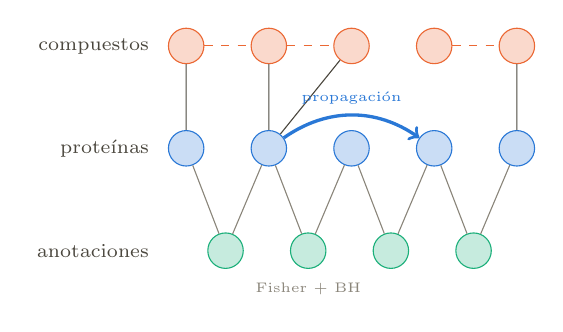
\begin{tikzpicture}
  \foreach \i in {0,...,4} \node[n=naranja] (c\i) at (\i*1.05,2.6) {};
  \foreach \i in {0,...,4} \node[n=azulo] (p\i) at (\i*1.05,1.3) {};
  \foreach \i in {0,...,3} \node[n=verde] (a\i) at (\i*1.05+.5,0) {};
  \node[l] at (-.35,2.6) {compuestos};
  \node[l] at (-.35,1.3) {proteínas};
  \node[l] at (-.35,0) {anotaciones};
  \draw[naranja,dashed] (c0)--(c1) (c1)--(c2) (c3)--(c4);
  \draw[tinta2] (c0)--(p0) (c1)--(p1) (c2)--(p1) (c4)--(p4);
  \draw[tenue] (p0)--(a0) (p1)--(a0) (p1)--(a1) (p2)--(a1) (p2)--(a2)
               (p3)--(a2) (p3)--(a3) (p4)--(a3);
  \node[font=\tiny\color{tenue},below=.05 of a1] {Fisher + BH};
  \draw[->,very thick,azulo] (p1) to[bend left=35] node[above,font=\tiny]{propagación} (p3);
\end{tikzpicture}\\[.6em]
{\scriptsize\color{tinta2}\NProteinas\ proteínas · \NEspecies\ organismos ·
\NPositivos\ enlaces positivos · \NAfiliaciones\ afiliaciones}
\end{columns}
\end{frame}

% ---------------------------------------------------------- 3 · camino v4
\begin{frame}{El camino con Claude, I: de v3 a v4}
\begin{columns}[T]
\column{.47\textwidth}
\begin{block}{Punto de partida}
\begin{itemize}\setlength\itemsep{.35em}\small
\item La misma métrica implementada \textbf{tres veces}, con tres resultados.
  Un bug en la pAUC (signo invertido, sin interpolar) sobrevivió meses.
\item Carpetas \texttt{v3}, \texttt{v4}, \texttt{v5}, \texttt{claude},
  \texttt{it0–it3}: nada decía qué las distinguía.
\item Una docena de carpetas de scripts nunca corridas completas; una celda de
  figuras apuntaba a un directorio borrado.
\end{itemize}
\end{block}
\column{.49\textwidth}
\begin{block}{Lo que armamos}
\begin{itemize}\setlength\itemsep{.35em}\small
\item \textbf{Un solo lugar} para el modelo y la métrica (\texttt{comun/}); el
  modelo sólo cambia con una prueba que lo justifique.
\item Formato fijo de notebook: el ciclo se lee en la celda de corrida; cada
  salida lleva el número de su notebook y un \texttt{meta.json}.
\item \textbf{Se recalculó todo} con la métrica corregida, contra una corrida
  independiente como control.
\item Decisiones escritas: el filtro de promiscuidad
  (\PromiscuosVcuatro\ compuestos, \PctAristasVcuatro\,\% de la capa) se aplica.
\end{itemize}
\end{block}
\end{columns}
\end{frame}

% -------------------------------------------------- 4 · camino este repo
\begin{frame}{El camino con Claude, II: la base codificada}
\begin{columns}[T]
\column{.56\textwidth}
\begin{enumerate}\setlength\itemsep{.45em}\small
\item[\color{azulo}\bfseries 1] \textbf{Acondicionar la base} para publicarla
  (siguiente diapositiva).
\item[\color{azulo}\bfseries 2] \textbf{Pruebas antes que resultados.}
  Encontraron cuatro fallas \emph{silenciosas}, todas iguales: un entero
  codificado comparado contra el texto que solía ser.
  \begin{itemize}\scriptsize
  \item \texttt{== "positive"} daba 0 filas: \NPositivos\ enlaces descartados sin error
  \item la pseudo-especie aportaba el 53\,\% de las pseudohuérfanas
  \end{itemize}
\item[\color{azulo}\bfseries 3] \textbf{Contrastar con v4}: \NComparadas\
  columnas, \NDiscrepancias\ discrepancias. Priorización idéntica
  (\NIdenticasGP/\NComparadasGP); control \ControlCoinciden/\NEspeciesOpt,
  $\Delta$AUC01 = \ControlDeltaMax.
\item[\color{azulo}\bfseries 4] \textbf{Entregables sin cifras a mano}, y
  corrida separada de figuras: \NFiguras\ figuras en $\sim$30\,s.
\end{enumerate}
\column{.42\textwidth}
\centering
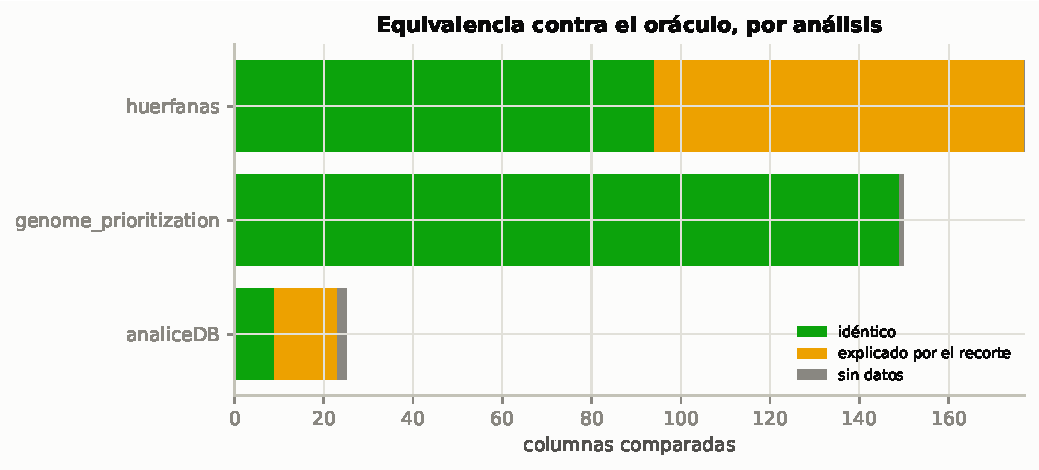
\includegraphics[width=\textwidth]{figuras/10_f01_equivalencia.pdf}\\
{\scriptsize\color{tinta2}Verde: idéntica a v4. Ámbar: cambio que el recorte
explica. Si el análisis toca la capa química, el recorte lo mueve; si no, no.}
\end{columns}
\end{frame}

% ------------------------------------------------- 5 · ocultar los nodos
\begin{frame}{Ocultar los nodos: la base que se puede publicar}
\begin{columns}[T]
\column{.32\textwidth}
\begin{block}{Recortar}
\small Se eliminan las componentes químicas sin ninguna bioactividad positiva:
no pueden aportar a la propagación.\\[.5em]
\cifra{\NCompuestosAntes\,$\to$\,\NCompuestosDespues}{compuestos (\PctCompuestosConservados\,\%); toda la evidencia positiva sobrevive}
\end{block}
\column{.32\textwidth}
\begin{block}{Codificar}
\small Todo identificador pasa a un entero en orden aleatorio (semilla
\SemillaCod). Los diccionarios quedan privados; ninguna especie se nombra.\\[.5em]
\cifra{\NCodigos}{identificadores en \NDiccionarios\ diccionarios}
\end{block}
\column{.32\textwidth}
\begin{block}{Empaquetar}
\small Las aristas se parten en dos \texttt{.csv.gz} de menos de 100\,MB, sin
subir el umbral de similitud (que costaba compuestos).\\[.5em]
\cifra{\NAristas}{aristas, completas}
\end{block}
\end{columns}
\vspace{1em}
{\small\color{tinta2}\textbf{El costo.} Se publica el tipo de organismo, que el
modelo usa: 3 de 16 son únicos en su combinación y quedan identificables. Y los
nombres de las anotaciones no se pueden reconstruir.}
\end{frame}

% ------------------------------------------- 6 · resultados priorizacion
\begin{frame}{Resultados I: priorizar un genoma sin su propia evidencia}
\begin{columns}[c]
\column{.55\textwidth}
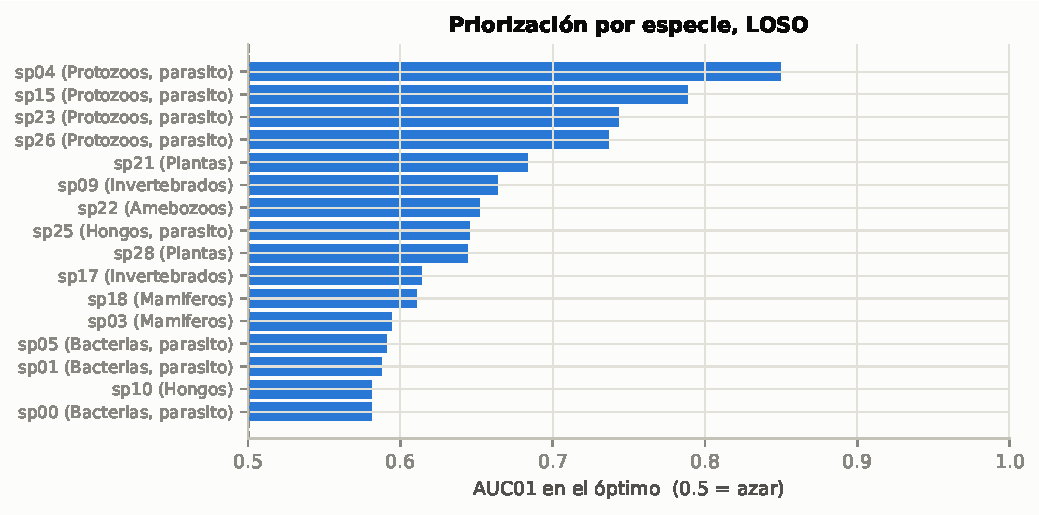
\includegraphics[width=\textwidth]{figuras/01_f03_auc01_por_especie.pdf}
\column{.43\textwidth}
\begin{itemize}\setlength\itemsep{.55em}\small
\item Supera al azar en los \textbf{\NSobreAzar} organismos; AUC01 mediana
  \AUCMediana\ (\AUCMin–\AUCMax).
\item Los \NProtozoosArriba\ primeros son los \NProtozoos\ \textbf{protozoos
  parásitos}.
\item Lo decide un solo parámetro, \textbf{$\beta$}: penalizar las categorías
  grandes. $\beta>0$ en \NBetaPositivo/\NEspeciesOpt\ óptimos; $\beta=1$ está
  \EnrBetaUno$\times$ sobrerrepresentado en el top-10.
\item El óptimo es una meseta: las 20 mejores combinaciones quedan a menos del
  \CaidaTopVeinteMax\,\% del máximo.
\end{itemize}
\end{columns}
\end{frame}

% ---------------------------------------------- 7 · resultados huerfanas
\begin{frame}{Resultados II: proponer el blanco de un compuesto huérfano}
\begin{columns}[T]
\column{.5\textwidth}
\small Se le borra toda la bioactividad a \NPseudo\ compuestos con un único
blanco conocido, y se lo busca desde su vecindario químico.
\begin{itemize}\setlength\itemsep{.45em}
\item Se recupera en el \textbf{\PctRecuperadas\,\%}. La causa está medida:
\item el \textbf{\PctSinSemilla\,\%} no tiene ningún vecino químico con blanco;
\item si la semilla comparte una anotación con el blanco: \textbf{\PctRecInformativa\,\%};
  si no, \PctRecNoInformativa\,\%.
\item El límite es la cobertura química, no el modelo: el techo va del
  \TechoMin\ al \TechoMax\,\% por organismo.
\end{itemize}
\column{.48\textwidth}
\centering
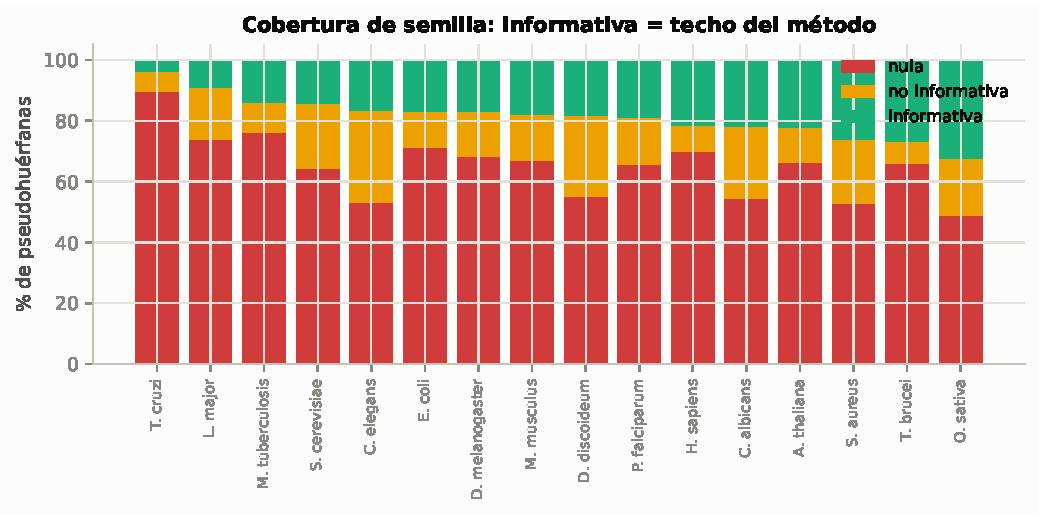
\includegraphics[width=\textwidth]{figuras/01_f03_semilla_por_especie.pdf}\\[.3em]
{\scriptsize\color{tinta2}Rojo: sin semilla. Ámbar: semilla sin anotación en común.
Verde: semilla informativa.}
\end{columns}
\end{frame}

% ------------------------------------ 8 · resultados semilla informativa
\begin{frame}{Resultados III: cuando hay semilla informativa}
\begin{columns}[c]
\column{.6\textwidth}
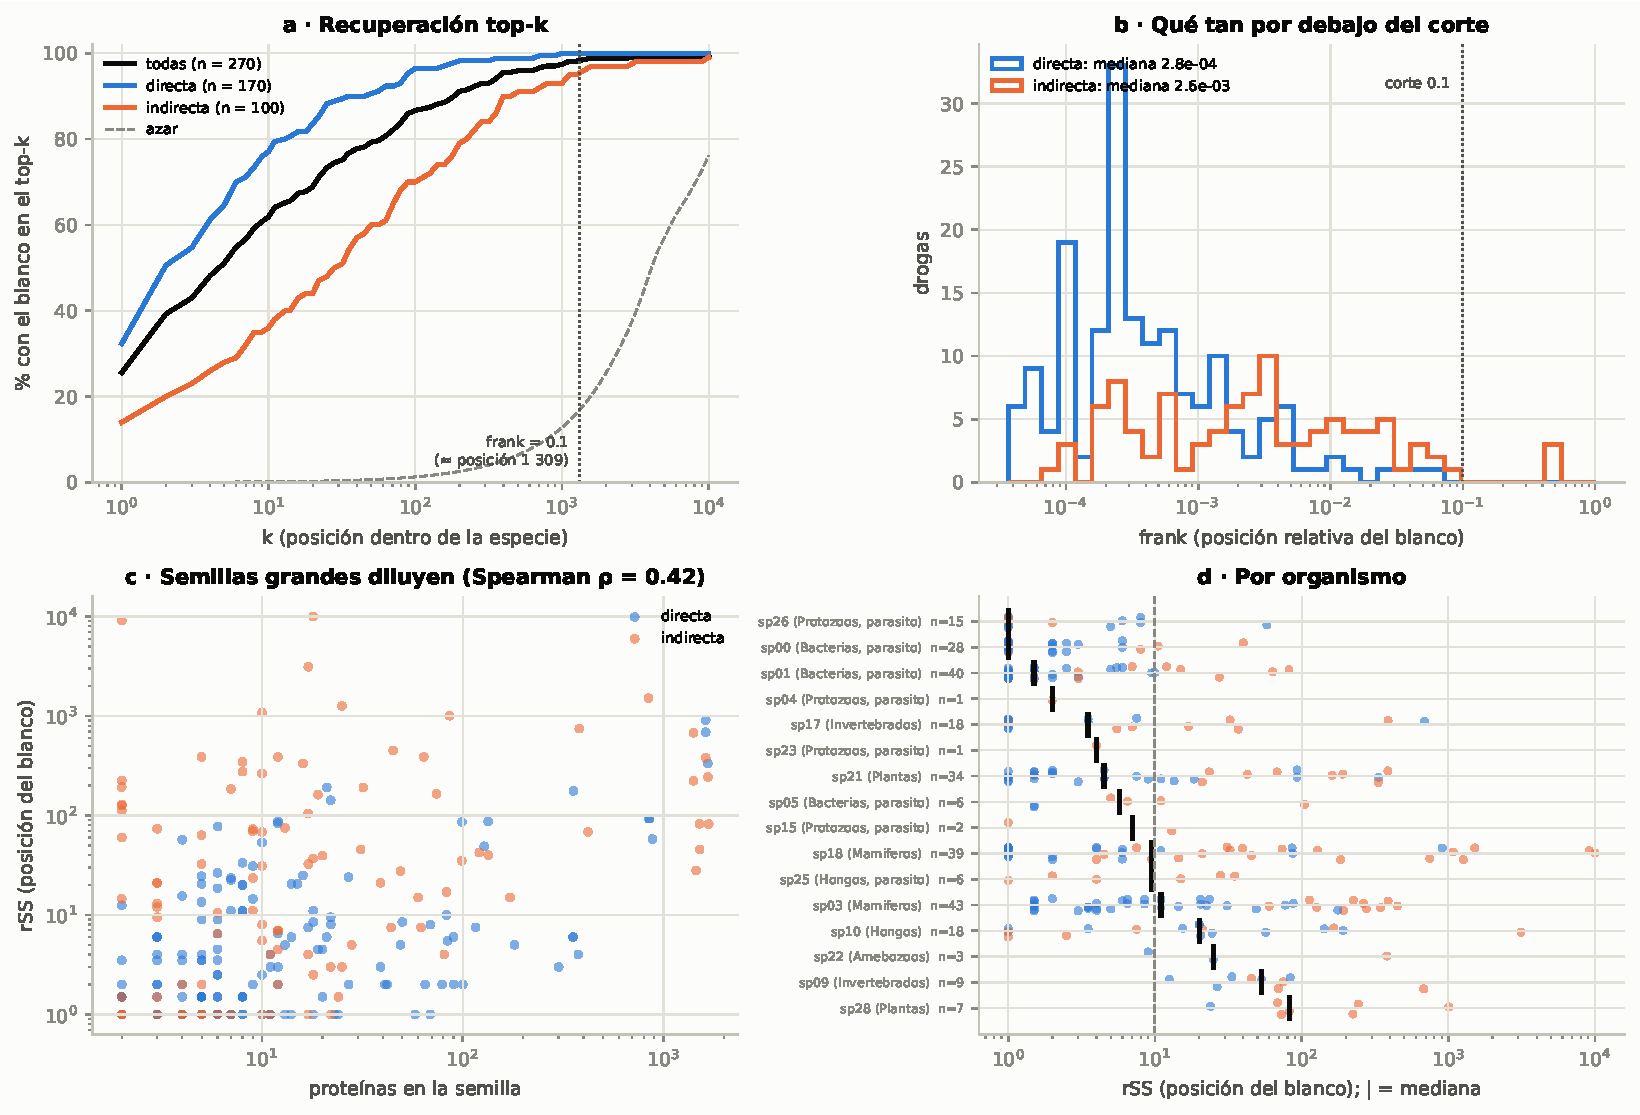
\includegraphics[width=\textwidth]{figuras/03_f05_semilla_informativa.pdf}
\column{.38\textwidth}
\small $\mathrm{frank}<0.1$ es quedar entre las primeras $\sim$\FrankCorteRank: no
discrimina. Con la posición exacta:
\begin{itemize}\setlength\itemsep{.45em}
\item \textbf{1.º} en el \PctInfTopUno\,\%, \textbf{top-10} en el
  \PctInfTopDiez\,\% (azar: \AzarTopDiez\,\%).
\item \textbf{Directa} (el vecino trae el blanco): mediana \RSSMedInfDirecta.
  \textbf{Indirecta} (sólo anotaciones): \RSSMedInfIndirecta.
\item Semillas grandes diluyen: $\rho=\RhoSemillaRSS$, positiva en
  \NOrgRhoPos/\NOrgRho\ organismos.
\end{itemize}
\end{columns}
\end{frame}

% --------------------------------------------------------------- 9 · cierre
\begin{frame}{Qué me llevo}
\begin{columns}[T]
\column{.48\textwidth}
\begin{block}{Del problema}
\begin{itemize}\setlength\itemsep{.4em}\small
\item La propagación prioriza genomas de los que no se sabe nada, y lo que la
  hace funcionar es penalizar las categorías grandes.
\item Para desorfanizar, el cuello de botella es la cobertura química: cuando
  hay semilla informativa, el blanco cae en el top-10 el \PctInfTopDiez\,\% de
  las veces.
\item Siguiente paso: ampliar la semilla (umbral de similitud por debajo de
  0.8, KEGG).
\end{itemize}
\end{block}
\column{.48\textwidth}
\begin{block}{Del trabajo con Claude}
\begin{itemize}\setlength\itemsep{.4em}\small
\item Las pruebas antes que los resultados: las fallas caras no lanzan
  excepciones.
\item Cada cifra se lee de una tabla; cada decisión queda escrita con la
  alternativa que se descartó (\texttt{PROVENANCE.md}).
\item Separar la corrida de las figuras: iterar sobre una figura cuesta
  segundos, no la corrida.
\end{itemize}
\end{block}
\end{columns}
\end{frame}

\end{document}
